\documentclass[handout, c,english]{beamer}
\usetheme{Frankfurt}
\usepackage[utf8]{inputenc}
\usepackage{natbib}
%\usepackage[french]{babel}
\usepackage[english]{babel}
\usepackage{listings}
\usepackage{hyperref}
\usepackage{tikz}
\usepackage{algorithm}
\usepackage[noend]{algpseudocode}
\usepackage{pgfplots}
\usepackage{comment}
\usepackage{todonotes}

%animations (for gifs)
\usepackage{animate}

%used to plot results
\usepackage{pgfplots}
\usepackage{pgfplotstable}

%customize itemize
\usetikzlibrary{positioning,calc,intersections,shapes.geometric}

\setbeamertemplate{footline}[frame number]


\title{IEEE ICTAI 2022}
\subtitle{Extending a Refinement Acting Engine for Fleet Management: Concurrency and Resources}
\author{Jérémy Turi, Arthur Bit-Monnot \\
jeremy.turi@laas.fr, abitmonnot@laas.fr}
\institute{\textit{LAAS-CNRS, Université de Toulouse, CNRS, INSA,} Toulouse, France}
\date{\today}

\begin{document}

\begin{frame}
\titlepage
\end{frame}

\begin{frame}
\frametitle{Outline}
\tableofcontents
\end{frame}

\AtBeginSection[]
{
  \begin{frame}
    \frametitle{Table of Contents}
    \tableofcontents[currentsection]
  \end{frame}
}

\section{Context}
\begin{frame}{People and Research subject}
    \begin{itemize}
        \item Personal brief
        \item Lab presentation
        \item Team presentation and research focus
    \end{itemize}
\end{frame}
\section{Motivation}
\begin{frame}{Deliberation in robotics} 
\end{frame}
\section{Contribution}
\subsection{OMPAS}
\begin{frame}{Features}
    \begin{columns}
        \begin{column}{0.5\textwidth}
            Basic RAE features:
            \begin{itemize}
                \item 
            \end{itemize}
        \end{column}
        \begin{column}{0.5\textwidth}
            OMPAS features:
            \begin{itemize}
                \pause
                \item Handle concurrency inside methods
                \pause
                \item Refinement guided by an HTN temporal planner
                \pause
                \item Custom Acting language to define acting domains
            \end{itemize}
        \end{column}
    \end{columns}
\end{frame}

\begin{frame}{Adaptation of the main algorithm}
    
\end{frame}

\subsection{SOMPAS}
\begin{frame}{Scheme OMPAS, a dedicated acting language}
    \begin{columns}
        \begin{column}{0.5\textwidth}
            What we want in the acting language
        \end{column}
        \begin{column}{0.5\textwidth}
            Features of the language
        \end{column}
    \end{columns}
\end{frame}

\begin{frame}{Concurrency and interruption}
    \begin{itemize}
        \item Extension of Scheme with a handle LValue
        \item Functions:
        \begin{itemize}
            \item async
            \item await
            \item interrupt
        \end{itemize}
    \end{itemize}
\end{frame}

\begin{frame}{Acting primitives}
    \begin{itemize}
    \pause
        \item exec-task: execute and monitor a task
    \pause
        \begin{itemize}
            \item primitive-task: request to the platform
            \item abstract-task: select a method and execute the operational model.
        \end{itemize}
    \pause
        \item read-state: return the value of a state-variable
        \item arbitrary
    \end{itemize}
\end{frame}

\begin{frame}{Resources}
    \begin{columns}
        \begin{column}{0.5\textwidth}
            Definition of a resource
        \end{column}
        \begin{column}{0.5\textwidth}
            Language interface:
            \begin{itemize}
                \item Define: new-resource
                \item Request: acquire
                \item End the usage: release
            \end{itemize}
        \end{column}
    \end{columns}
\end{frame}

\begin{frame}{More advanced features and programming constructs}
    Constructs inspired by what other acting systems and languages feature:
    \begin{itemize}
        \item monitor, wait-for
        \item par, race
        \item others
    \end{itemize}
\end{frame}

\begin{frame}[t,fragile]{Defining $A_\Delta$ with Scheme OMPAS (SOMPAS)}
    \setlength{\leftmargini}{0pt}
    \begin{columns}
        \begin{column}{0.5\textwidth}
            \begin{itemize}
                \footnotesize
                \item Task (label, typed parameters):
                \tiny
                \begin{lstlisting}
(def-task t_process_package
    '(?p package))
                \end{lstlisting}
                \footnotesize
                \pause
                \item Method (label, typed parameters, pre-conditions, body):
                \tiny
                \begin{lstlisting}
(def-method m_process_to_do_r
'((:task t_process_package)
  (:params (?p package))
  (:pre-conditions
    (!= (package.processes_list ?p)
        nil)))
  (:body
    (do
     (define ?m ...)
     (t_process_on_machine ?p ?m)
     (t_process_package ?p)))))    
                \end{lstlisting}
            \end{itemize}
        \end{column}
\pause
        \begin{column}{0.5\textwidth}
            \begin{itemize}
                \pause
            \footnotesize
            \item State-function (label, typed parameters \& result):
            \tiny
            \begin{lstlisting}
(def-state-function
at
'(?r robot)
'(?l location))
            \end{lstlisting}
            \pause
            \footnotesize
            \item Action (label, typed parameters):
            \tiny
            \begin{lstlisting}
(def-action pick '(?r robot))
                \end{lstlisting}
            \end{itemize}

    \pause
            ~
        \normalsize
        Others:
        
        \textit{lambda, type, constant}
        \end{column}

    \end{columns}
\end{frame}
\section{Model example for a factory simulator}

\begin{frame}[fragile]{Multi-agent model}
    \begin{columns}
        \begin{column}{0.5\textwidth}
            \centering
            \includegraphics[width = 0.3\textwidth]{images/godot/package.png}
            
            \Large $\times n$
        \end{column}
        \begin{column}{0.5\textwidth}
            \centering
            \includegraphics[width = 0.3\textwidth]{images/godot/robot_texture.png}
            
            \LARGE $\times m$
        \end{column}
    \end{columns}
\pause
~~
\centering
        Modelled with a unique high-level task:
        \setlength{\leftmargini}{0pt}
        \lstset{columns=fullflexible}
        \small
    \begin{lstlisting}[language = lisp]
(do
    ;declare robots and machines as resources
    (mapf new-resource (instances robot))
    (mapf new-resource (instances machine))
    ;process all packages
    (define h1 (async (t_process_packages)))
    ;monitor in parallel batteries of robots
    (define h2 (async (t_check_rob_bat)))
    (await h1)) ;await that all packages are processed
    \end{lstlisting}    
\end{frame}

\begin{frame}{Running example for several packages}
    \centering

    \includegraphics[width = 0.8\textwidth]{images/gobot-multi-robot.png}
    \Large

    Video example: \href{https://youtu.be/8z2aUsWTq4k}{https://youtu.be/8z2aUsWTq4k}
\end{frame}


% Presentation des problématiques traités,
% Expressivité des modèles => 
% Greedy => facilement faisable avec d'autres implémentations de RAE
% Advanced => plus compliqué à faire avec les autres implémentations de Python => 
% Ici pas de garantie de "no race condition" à l'accès d'une ressource
\begin{frame}[fragile]{Validation on job shop problems}
%\centering
%Outline the features of the new system and the language
%Organiser le passage de plusieurs tâches sur des machines.
%transport des paquets entre les machines
Job shop : $n$ packages should be processed on $m$ machines

Robotic system mission:
\begin{itemize}
    \pause
    \item Schedule packages passages on machines to optimize the total processing time.
    \pause
    \item Take into account robot displacement times. 
\end{itemize}

\end{frame}


\begin{frame}{Definition of several reactive behaviors for the robotic agent}
    Several resource allocation strategies: 
    \begin{itemize}
        \pause
        \item Greedy: acquire random robot
        \pause
        \item Advanced: acquire first available robot
        \pause
        \item ALRPTF: Advanced+prority to package with \textit{Longest Remaining Processing Time}
    \end{itemize}
\end{frame}




\newcommand{\calcrowmean}{
    \def \rowmean{0}
    \pgfmathparse{\pgfkeysvalueof{/pgfplots/table/summary statistics/end index}-\pgfkeysvalueof{/pgfplots/table/summary statistics/start index}+1}
    \edef\numberofcols{\pgfmathresult}
            % ... loop over all columns, summing up the elements
    \pgfplotsforeachungrouped \col in {1,2,3,4,5,6,7,8,9,10}% in {\pgfkeysvalueof{/pgfplots/table/summary statistics/start index},...,\pgfkeysvalueof{/pgfplots/table/summary statistics/end index}}
    {
        
        \typeout{col = \col}
        
        \pgfmathparse{\rowmean+\thisrowno{\col}/\numberofcols}
        \edef \rowmean{\pgfmathresult}
    }
}
\newcommand{\calcstddev}{
    \def\rowstddev{0}
    \calcrowmean
    \pgfplotsforeachungrouped \col in {1,2,3,4,5,6,7,8,9,10}
    % {\pgfkeysvalueof{/pgfplots/table/summary statistics/start index},...,\pgfkeysvalueof{/pgfplots/table/summary statistics/end index}}
    {
        \pgfmathparse{\rowstddev+(\thisrowno{\col}-\rowmean)^2/(\numberofcols-1)}
        \edef\rowstddev{\pgfmathresult}
    }
    \pgfmathparse{sqrt(\rowstddev)}
}
\newcommand{\calcstderror}{
    \calcrowmean
    \calcstddev
    \pgfmathparse{sqrt(\rowstddev)/sqrt(\numberofcols)}
}

\pgfplotstableset{
    summary statistics/start index/.initial=1,
    summary statistics/end index/.initial=10,
    create col/mean/.style={
        /pgfplots/table/create col/assign/.code={% In each row ... 
            \calcrowmean
            \pgfkeyslet{/pgfplots/table/create col/next content}\rowmean
        }
    },
    create col/standard deviation/.style={
        /pgfplots/table/create col/assign/.code={% In each row ... 
            \calcstddev
            \pgfkeyslet{/pgfplots/table/create col/next content}\pgfmathresult
        }
    },
    create col/standard error/.style={
        create col/assign/.code={% In each row ... 
            \calcstderror
            \pgfkeyslet{/pgfplots/table/create col/next content}\pgfmathresult
        }
    }
}

\pgfplotstableset{
    create on use/mean/.style={create col/mean},
    create on use/stddev/.style={create col/standard deviation},
    create on use/stderror/.style={create col/standard error}
}



\begin{frame}[fragile]{Comparison of reactive strategies on job shop problems}

    \begin{tikzpicture}
        \begin{axis}[
                    /pgf/number format/.cd,
                        use comma,
                    height = 6cm,
                    width = \linewidth,
                    ymajorgrids,
                    ylabel={Time in seconds},
                    xlabel={Problems},
                    ymin = 0,
                    ymax= 220,
                    ybar=0pt,
                    bar width=12pt,
                    enlarge x limits = 0.3,
                    nodes near coords,
                    point meta=explicit symbolic,
                    scatter/position=absolute,
                    every node near coord/.style={
                            at={(\pgfkeysvalueof{/data point/x},1.8)},
                            anchor=south,
                        },
                    bar shift=0pt,
                    xtick={0,1,2,3},
                    xticklabels={p1,p2,p3,p4},
                    x tick label style={rotate=45,anchor=east},
                    legend cell align = {left},
                    legend pos = north west,
                    legend image post style={scale=0.4},
                    legend style={font = \footnotesize},
                ]
        \addplot+[bar shift = -12pt]
        plot[
                %smooth,
                error bars/.cd,
            y dir=both,
            y explicit
        ]
        table[
                x=Problem,
                y=mean,
                y error=stderror
        ]
        {datas/jobshop_greedy.dat};
        \addplot+
        [bar shift = +0pt]
        plot[
                %smooth,
                error bars/.cd,
            y dir=both,
            y explicit
        ]
        table[
                x=Problem,
                y=mean,
                y error=stderror
        ]
        {datas/jobshop_advanced.dat};
        \addplot+[bar shift = +12pt]
        plot[
                %smooth,
                error bars/.cd,
            y dir=both,
            y explicit
        ]
        table[
                x=Problem,
                y=mean,
                y error=stderror
        ]
        {datas/jobshop_advanced_lrptf.dat};
    
        \legend{
                    Greedy,
                    Advanced,
                    ALRPTF}
    \end{axis}
    \end{tikzpicture}
    
    \pause

    Future work: improve the system with \textbf{anticipation} capabilities \textbf{(planning)}
  
\end{frame}
\section{Conclusion \& perspectives (2 min)}
\begin{frame}[c]{Conclusion}
    OMPAS, an acting system:
    \pause
        \begin{itemize}
            \item Implementing RAE
            \item Capable of using planning to guide the refinement of task
            \item Using a custom acting language
            \item From with descriptive models can be extracted
        \end{itemize}    
\end{frame}

\begin{frame}[c]{Perspectives}
    \begin{itemize}
        \item Extraction rules for all primitives of the language
        \pause
        \item Test on more complex problems than graph exploration
        \pause
        \item Compare with other techniques (UPOM \cite{patraIntegratingActingPlanning2020}, Run-Lazy-Refineahead \cite{bansod2021integrating},\dots)
        \pause
        \item Take into account error handling from operational model into the chronicle encoding
    \end{itemize}
\end{frame}
%\section{Introduction}
\subsection{Deliberation for logistic}

\begin{frame}{Scientific interests of the authors}
    \centering
\begin{columns}
    \begin{column}{0.5\textwidth}
        Deliberation techniques applied to robotics:
        \begin{itemize}
            \item Hierarchical and temporal planning techniques.
            \item Robotic architecture.
            \item Cooperation in complex and large environment.
        \end{itemize}
    \end{column}
    \begin{column}{0.5\textwidth}
        Focus on deliberation in logistic problems: 
        \begin{itemize}
            \item Scheduling,
            \item Robot control,
            \item Fleet Management,
            \item Resource allocation.
        \end{itemize}
        \includegraphics[width = \textwidth]{images/logisticsolutions.jpg}
    \end{column}
\end{columns}

\end{frame}

\begin{frame}{Factory simulator for logistic problems}
    GobotSim: A new simulator for logistic problems.
    \begin{columns}
        \begin{column}{0.5\textwidth}
            Compaired to existing simulators:
            \begin{itemize}
                \item RoboCup: Manipulation, cooperation
                \item Craft-bots: Exploration, resource gathering
            \end{itemize}
        \end{column}
        \begin{column}{0.5\textwidth}
            Environment: 
        \end{column}
    \end{columns}
\end{frame}

\subsection{Single agent scenario}


\begin{frame}{Simple scenario: one package}
    \centering
    \begin{columns}
        \begin{column}{0.5\textwidth}
            \centering
            \includegraphics[width = 0.5\textwidth]{images/godot/package.png}
            
            \LARGE \emph{$\times 1$}
        \end{column}
        \begin{column}{0.5\textwidth}
            \centering
            \includegraphics[width = 0.5\textwidth]{images/godot/robot_texture.png}
            
            \LARGE \emph{$\times 1$}
        \end{column}
    \end{columns}
\end{frame}

\begin{frame}{Definition of a robotic agent}

    \begin{columns}[T]
        \begin{column}{0.3\textwidth}
            An entity

            ~

            \includegraphics[width = 0.7\textwidth]{images/icons8-robot-gustav-500.png}
        \end{column}
        \begin{column}{0.7\textwidth}
            \center Capable of :
            \pause
            \begin{enumerate}
                \item Perceiving its environment
                \pause
                \item Modifying its environment (actions)
                \pause
                \item \textbf{Deliberating:} Reasoning about its \textbf{skills} in order to fulfill a goal
            \end{enumerate}
        \end{column}
    \end{columns}

 
\end{frame}

\begin{frame}{Hierarchical operational models to represent the capabilities of an agent}

\begin{columns}[T]
    \begin{column}{0.55\textwidth}

        \begin{itemize}
            \item Elementary capabilities : move, pick, place, \dots
            \pause
            \item Skills : executable programs (operational models): transport, process \dots
            \pause
            \item Agent behavior = composition of skills
        \end{itemize}
        
        ~
        \pause
        Acting domain \textbf{$A_\Delta (A, T, M_t)$}: Hierarchical operational models
        \small
        \pause
        \begin{itemize}
        
        
         \item[$A$] : commands
         \pause
         \item[$T$] : tasks
         \pause
         \item[$M_t$] : methods: pre-conditions, body (operational model)
         
     \end{itemize}
    \end{column}
    \pause
    \begin{column}{0.45\textwidth}
        \begin{figure}
            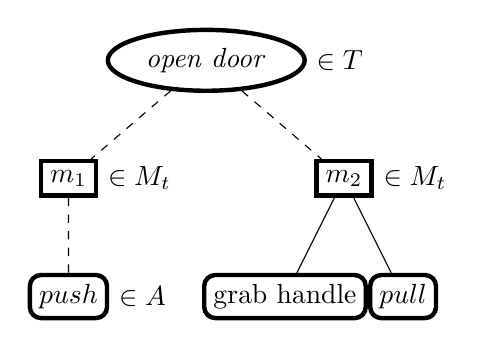
\begin{tikzpicture}
                \node[draw,ellipse, ultra thick] (t) {\textit{open door}} [sibling distance = 3.5cm]
                  child {node[draw, ultra thick] (m1) {$m_1$} edge from parent [dashed]
                  child {node[draw,rounded corners, ultra thick, solid] (a1) {$push$} edge from parent
                  }} 
                  child {node[draw, ultra thick] (m2) {$m_2$} edge from parent [dashed] [sibling distance = 1.5cm]
                  child {node[draw, rounded corners, solid, ultra thick] (a2) {grab handle} edge from parent [solid]}
                  child {node[draw, rounded corners, solid, ultra thick] {$pull$} edge from parent [solid]}};
                \node[right = 0em of t] {$\in T$};
                \node[right = 0em of m1] {$\in M_t$};
                \node[right = 0em of m2] {$\in M_t$};
                \node[right = 0em of a1] {$\in A$};

            \end{tikzpicture}
            \caption{Example of hierarchy for the \textit{task} \textit{open door}}

            
        \end{figure}
    \end{column}
\end{columns}
    
\end{frame}

\begin{frame}{Deliberate using hierarchical operatinal models with the Refinement Acting Engine (RAE)\footnote{Automated Planning and Acting \cite{ghallabAutomatedPlanningActing2016}}}
    RAE features:
    \begin{itemize}
        \item Monitor command and task execution in parallel.
        \item Refine tasks at runtime to select a suitable method with its parameters depending on the context
        
        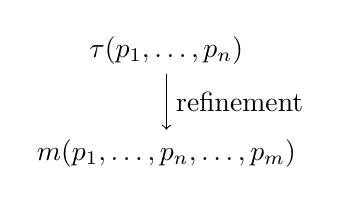
\begin{tikzpicture}
            \node[] (task) {$\tau(p_1,\dots,p_n)$};
            \node[below = 2em of task] (method) {$m(p_1,\dots,p_n, \dots, p_m)$};
            \path[->] (task) edge node[right, midway] {refinement} (method);
        \end{tikzpicture}
    \end{itemize}    
\end{frame}
    

\begin{frame}{Refinement Acting Engine algorithms}
    \begin{columns}[T]
  
        \begin{column}{0.65\textwidth}
            
            Algorithms:
            \small
            \begin{itemize}
                \setlength{\leftmargini}{-1pt}
                \onslide<2->
                \item \textbf{Main:} 
                \begin{itemize}
                    \item Receive $\tau$ (task or event);
                    
                    add it to the \textbf{agenda} (ongoing tasks)
                    \onslide<3->
                    \item Refine $\tau$: \textbf{Select} an applicable method $m$ for $\tau$
                    \onslide<4->
                    \item \textbf{Progress} $m$
                \end{itemize}
                \onslide<5->
                \item \textbf{Progress:}
                    \begin{itemize}
                        \onslide<6->
                        \item Monitor execution of $m$.
                        \onslide<7->
                        \item Refine subtasks in $m$.    
                        \onslide<8->
                        \item Monitor execution of subtasks.
                        \onslide<9->
                        \item \textbf{Retry} $\tau$ in case of \emph{failure}:
                    
                    Call \textbf{Select} to get a new method;
                    
                    \textbf{Progress} the new method.
                    \end{itemize}
            \end{itemize}
        \end{column}
        \begin{column}{0.35\textwidth}
            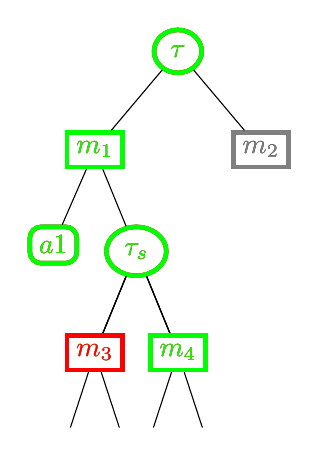
\begin{tikzpicture}
                \onslide<2>
                \node[draw,ellipse, ultra thick] (t) {$\tau$};
                \onslide<3-9>
                \node[draw,ellipse, ultra thick, color = orange] (t) {$\tau$};
                \onslide<10>
                \node[draw,ellipse, ultra thick, color = green] (t) {$\tau$};
                \onslide<3>
                \node[draw, ultra thick, below= 2em of t, xshift = -3em] (m1) {$m_1$};
                \node[draw, ultra thick, below= 2em of t, xshift = 3em] (m2) {$m_2$};
                \onslide<4->
                \node[draw, ultra thick, below= 2em of t, xshift = -3em, color = orange] (m1) {$m_1$};
                \node[draw, ultra thick, below= 2em of t, xshift = 3em, color = gray] (m2) {$m_2$};
                \onslide<10>
                \node[draw, ultra thick, below= 2em of t, xshift = -3em, color = green] (m1) {$m_1$};
                \onslide<3->
                \path[-] (t) edge (m1) (t) edge (m2);
                \onslide<5>
                \node[draw,rounded corners, ultra thick, solid, below = 2em of m1, xshift = -1.5em] (a1) {$a1$};
                \onslide<6>
                \node[draw,rounded corners, ultra thick, solid, below = 2em of m1, xshift = -1.5em, color = orange] (a1) {$a1$};
                \onslide<7->
                \node[draw,rounded corners, ultra thick, solid, below = 2em of m1, xshift = -1.5em, color = green] (a1) {$a1$};
                \onslide<5-7>
                \node[draw,ellipse, ultra thick, solid, below = 2em of m1, xshift = 1.5em] (t2) {$\tau_s$};
                \onslide<8->
                \node[draw,ellipse, ultra thick, solid, below = 2em of m1, xshift = 1.5em, color = orange] (t2) {$\tau_s$};
                \onslide<10>
                \node[draw,ellipse, ultra thick, solid, below = 2em of m1, xshift = 1.5em, color = green] (t2) {$\tau_s$};
  
  
                \onslide<5->
                \path[-] (m1) edge (a1) (m1) edge(t2);
  
  
                \onslide<7>
                \node[draw, ultra thick, below = 2em of t2, xshift = -1.5em] (m3) {$m_3$};
                \node[draw, ultra thick, below = 2em of t2, xshift = 1.5em] (m4) {$m_4$};
                \path[-] (t2) edge  (m3) (t2) edge (m4);
                
                \onslide<8>
                \node[draw, ultra thick, below = 2em of t2, xshift = -1.5em, color = orange] (m3) {$m_3$};
                \node[draw, ultra thick, below = 2em of t2, xshift = 1.5em, color = gray] (m4) {$m_4$};
                \path[-] (t2) edge  (m3) (t2) edge (m4);
  
                \onslide<9->
                \node[draw, ultra thick, below = 2em of t2, xshift = -1.5em, color = red] (m3) {$m_3$};
                \node[draw, ultra thick, below = 2em of t2, xshift = 1.5em, color = orange] (m4) {$m_4$};
                \path[-] (t2) edge  (m3) (t2) edge (m4);
                \onslide<10>
                \node[draw, ultra thick, below = 2em of t2, xshift = 1.5em, color = green] (m4) {$m_4$};
                
                \onslide<8->
                \node[below = 2em of m3, xshift = -1em] (e3) {};
                \node[below = 2em of m3, xshift = 1em] (e4) {};
                \path[-] (m3) edge  (e3) (m3) edge (e4);
  
                \onslide<8->
                \node[below = 2em of m4, xshift = -1em] (e5) {};
                \node[below = 2em of m4, xshift = 1em] (e6) {};
                \path[-] (m4) edge  (e5) (m4) edge (e6);
      
            \end{tikzpicture}
        \end{column}
    \end{columns}    
\end{frame}

\begin{frame}{RAE models for one package and one robot}
    \begin{itemize}
        \item Run example.
        \item High-level models.
    \end{itemize}
\end{frame}

\subsection{Multi-agent scenario}

\begin{frame}{Several packages?}
    \begin{columns}
        \begin{column}{0.5\textwidth}
            \centering
            \includegraphics[width = 0.5\textwidth]{images/godot/package.png}
            
            \Large $\times n$
        \end{column}
        \begin{column}{0.5\textwidth}
            \centering
            \includegraphics[width = 0.5\textwidth]{images/godot/robot_texture.png}
            
            \LARGE $\times m$
        \end{column}
    \end{columns}
    
    In function of n and m, deliberation must:
    \begin{itemize}
        \item Schedule package passage on machines
        \item Allocate package displacement tasks to robots
        \item Monitor the robots' batteries 
    \end{itemize}
\end{frame}

\begin{frame}{How to deliberate with multiple agents in parallel?}
    \begin{columns}
        \begin{column}{0.45\textwidth}
            RAE shortcomings:
            \begin{itemize}
                \item Progression of tasks relies on Round Robin
                \item Methods limited to a sequence of actions
                \item Difficulties to integrate sound planning from operational models due to implementation in Python.
            \end{itemize}
        \end{column}
        $\rightarrow$
        \pause
        \begin{column}{0.45\textwidth}
            Adapt RAE for multi-agents to
            \begin{itemize}
                \item Deal with concurrency
                \item Improve the interleaving of parallel tasks
                \item Reason on shared resources to optimize the overall process
            \end{itemize}
        \end{column}
    \end{columns}
\end{frame}

\begin{frame}{GobotSim environment}
\begin{columns}
\begin{column}{0.4\textwidth}
    \begin{figure}[tp]
        \includegraphics[width=\linewidth]{images/gobot-rae.png}
    \end{figure}
\end{column}
\begin{column}{0.5\textwidth}
    Machines
    \begin{itemize}
        \item Processing : does a predefined list of process for packages
        \item Input: generate packages
        \item Output: gather fully processed packages
    \end{itemize}
    Robots : manipulate packages
    \begin{itemize}
        \item commands: move, pick, place,\dots
        \item recharge at recharge areas
    \end{itemize}
\end{column}
\end{columns}
\end{frame}

\begin{frame}[fragile]{OMPAS models for GobotSim}
\begin{columns}
    \begin{column}{0.5\textwidth}
        \begin{itemize}
            \item High-level goal: process all packages in the environment
            \item Body of the unique method of the high-level task.
            \setlength{\leftmargini}{0pt}

            \tiny
        \begin{lstlisting}
(do
(mapf new-resource (instance robot))
(mapf new-resource (instance machine))
(define h1 (async (t_process_packages)))
(define h2 (async (t_check_rob_bat)))
(await h1))
        \end{lstlisting}    
        \end{itemize}


        
    \end{column}
    \begin{column}{0.5\textwidth}
Role of the acting engine : 
\begin{itemize}
\item Schedule package passage on machines
\item Allocate package displacement tasks to robots
\item Monitor the robots' batteries 
\end{itemize} 
\end{column}
\end{columns}

\end{frame}


\begin{frame}{The scope of the paper}
    Adaptation of a Refinement acting engine (RAE) for multi-agents to
    \begin{itemize}
        \item Deal with concurrency
        \item Improve the interleaving of parallel tasks
        \item Reason on shared resources to optimize the overall process
    \end{itemize}
\end{frame}

%\section{Deliberative agent (7 min)}

\begin{frame}{What is an agent}

    \begin{columns}[T]
        \begin{column}{0.3\textwidth}
            A robotic agent

            ~

            \includegraphics[width = 0.7\textwidth]{images/icons8-robot-gustav-500.png}
        \end{column}
        \begin{column}{0.7\textwidth}
            \center capable of :
            \pause
            \begin{enumerate}
                \item Perceiving its environment
                \pause
                \item Modifying its environment (actions)
                \pause
                \item \textbf{Deliberating:} Reasoning about its \textbf{skills} in order to fulfill a goal
            \end{enumerate}
        \end{column}
    \end{columns}

 
\end{frame}

\begin{frame}{Represent the skills of an agent}

\begin{columns}[T]
    \begin{column}{0.6\textwidth}

        Robot behavior = \textbf{operational model}:
        \begin{itemize}
            \item Executable program
            \item General purpose language
        \end{itemize}
        
        ~

        
        Acting domain \textbf{$A_\Delta (A, T, M_t)$}: Hierarchical operational models
        
                \begin{itemize}
        
        
         \item[$A$] \textit{(low-level skills)}: primitive tasks
         \pause
         
         \textit{\footnotesize(move, grasp, look)}
         \pause
         \item[$T$] \textit{(high-level skills)}: abstract tasks
         \pause

         \textit{\footnotesize(set the table, prepare a coffee)}
         \pause
         \item[$M_t$] \textit{("Know how")}: methods (operational models)

         
     \end{itemize}
    \end{column}
    \begin{column}{0.45\textwidth}
        \begin{figure}
            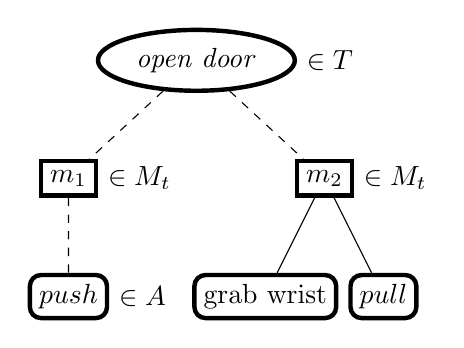
\begin{tikzpicture}
                \node[draw,ellipse, ultra thick] (t) {\textit{open door}} [sibling distance = 3.25cm]
                  child {node[draw, ultra thick] (m1) {$m_1$} edge from parent [dashed]
                  child {node[draw,rounded corners, ultra thick, solid] (a1) {$push$} edge from parent
                  }} 
                  child {node[draw, ultra thick] (m2) {$m_2$} edge from parent [dashed] [sibling distance = 1.5cm]
                  child {node[draw, rounded corners, solid, ultra thick] (a2) {grab wrist} edge from parent [solid]}
                  child {node[draw, rounded corners, solid, ultra thick] {$pull$} edge from parent [solid]}};
                \node[right = 0em of t] {$\in T$};
                \node[right = 0em of m1] {$\in M_t$};
                \node[right = 0em of m2] {$\in M_t$};
                \node[right = 0em of a1] {$\in A$};

            \end{tikzpicture}
            \caption{Example of hierarchy for the \textit{task} \textit{open door}}

            
        \end{figure}
    \end{column}
\end{columns}
    
\end{frame}
\begin{frame}{Refinement Acting Engine (RAE)\cite{ghallabAutomatedPlanningActing2016} : Deliberation algorithms using hierarchical operational models}
\begin{columns}
    \begin{column}{0.35\textwidth}
    \pause
    \setlength{\leftmargini}{-1pt}
    %\setlength{\parsep}{1pt}
    %\setlength{\parskip}{0pt}
    RAE features:
    \small
    \begin{itemize}
        \item Perform multiple tasks in parallel
        \pause
        \item Automated deliberation: Refinement of task
        \begin{itemize}
            \setlength{\leftmargini}{-1pt}
            \pause
            \item Refinement of task into a method
            \pause
            \item Instantiating of \textbf{arbitrary} variables
        \end{itemize}
    \end{itemize}
    \end{column}
    \begin{column}{0.65\textwidth}
        Algorithms:
        \small
        \begin{itemize}
            \setlength{\leftmargini}{-1pt}
            \item \textbf{Main:} 
            \begin{itemize}
                \item Receive $\tau$ (task or event);
                
                add it to the \textbf{agenda} (ongoing tasks)
                \pause
                \item Refine $tau$: \textbf{Select} an applicable method $m$ for $\tau$
                \pause
                \item \textbf{Progress} $m$
            \end{itemize}
            \item \textbf{Progress:}
                \begin{itemize}
                \item Monitor execution of $m$.
                \item Refine subtasks in $m$.    
                \item Monitor execution of subtasks.
                \item \textbf{Retry} $\tau$ in case of \emph{failure}:
                
                Call \textbf{Select} to get a new method;
                
                \textbf{Progress} the new method.
                \end{itemize}
                \pause
        \end{itemize}
    \end{column}
\end{columns}

    
\end{frame}

\begin{frame}{Improve the refinement using planning}
    \begin{center}
        
    Role of Select:

    ~

    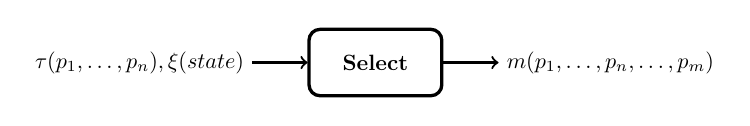
\begin{tikzpicture}[thick,scale=0.8, every node/.style={scale=0.8}]
    \node[draw = black, very thick,
        minimum width = 6em,
        minimum height = 3em,
        rounded corners,
        text = black,
        align=center,] (F) at (0,0) {\textbf{Select}};
        
    \pause
    \node[left= 2em of F] (i) {\textbf{$\tau(p_1,\dots,p_n), \xi (state)$}};
    \node[right= 2em of F] (o) {\textbf{$m(p_1, \dots, p_n,\dots,p_m)$}};
    \pause
    \path[->]
    (i) edge (F)
    (F) edge (o);

    \end{tikzpicture}
    

    %$Select(\tau, p_1,\dots,p_n) \rightarrow \{m_s, p_1, \dots, p_n,\dots,p_m\}$

    \end{center}

    Techniques:
    \begin{itemize}

    \item Greedy (Basic RAE functioning): arbitrary applicable method
    \pause
    
    \underline{Problem:} Does not take into account future refinements (can lead into dead-locks)
    \pause
    \item \textbf{look-ahead(planning)} : capacity to project the system from the current state to possible future state

    \end{itemize}
\end{frame}
\begin{frame}{How to use planning in RAE}
    %Make a high-level choice based on future choices the agent will have to make and its own capabilities to modify its environment.
    Requires:
    \begin{itemize}
        \item A planner
        \item Descriptive model of the agent skills : describes the set of states that may result from performing tasks.
    \end{itemize} 

    Descriptive models shortcomings:
    \begin{itemize}
        \item Made limited dedicated languages: PDDL \cite{foxPDDL2ExtensionPDDL2003}, ANML \cite{smith2008anml},\dots
        \item operational model $\not\equiv$ descriptive model $\rightarrow$ Harder design
    \end{itemize}

    ~
    
    \centering
    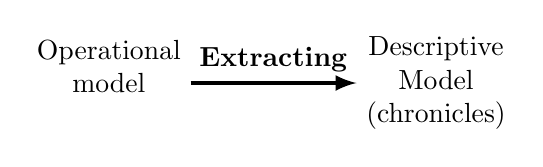
\begin{tikzpicture}
        \node[align = center] (O) {Operational\\ model \\};
        \node[right=6em of O, align = center] (D) {Descriptive\\ Model \\(chronicles)};
        \draw[-latex, ultra thick] (O.east)-- node[above, midway] (c) {\textbf{Extracting}} (D.west);
    \end{tikzpicture}

    Plan with \textbf{Aries} (hierarchical LCP\cite{bit-monnotConstraintBasedEncodingDomainIndependent2018} extension):

\end{frame}

\begin{frame}[c]{An analyzable acting language to extract descriptive models}
    \begin{columns}[c]
        \begin{column}{0.45\textwidth}
            Acting language Requirements:
            \begin{itemize}
                \item General purpose language
                \item Identified and simple semantic
            \end{itemize}
        \end{column}
        \begin{column}[c]{0.1\textwidth}
            \centering
            $\rightarrow$
        \end{column}
        \begin{column}{0.5\textwidth}
            Lisp dialect (Scheme variant) \cite{moretti1979lambda}

            Perks:
            \begin{itemize}
                \item Few primitives
                \item Immutable
                \item Functional
                \item Pure
            \end{itemize}
        \end{column}
    \end{columns}
\end{frame}

\begin{frame}{Synthesis of the proposition}
    \pause
        \centering
        Task refinement guided by planning:

        ~
        
        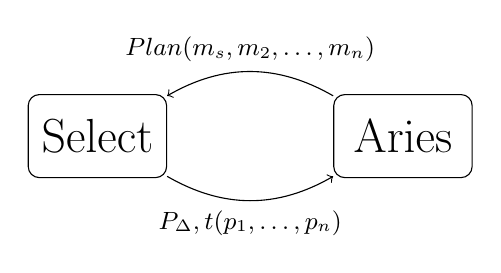
\begin{tikzpicture}
            \node[draw,
            rounded corners,
            minimum width = 5em,
            minimum height = 3em] (select) {\LARGE Select};
            \node[draw,
            rounded corners,
            right = 6em of select,
            minimum width = 5em,
            minimum height = 3em] (aries) {\LARGE Aries};
            \path[->, every node/.style={font=\sffamily\small}]
            (select) edge[bend right] node [right, below] {$P_\Delta, t(p_1,\dots,p_n)$} (aries)
            (aries) edge[bend right] node [right, above] {$Plan(m_s, m_2,\dots,m_n)$} (select)
            ;
        \end{tikzpicture}

        ~
    
        Planning domain extraction from operational models:

        ~

        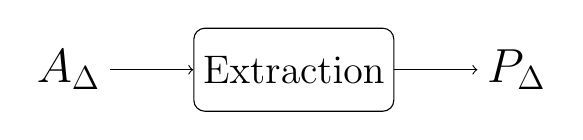
\begin{tikzpicture}
            \node (acting) {\LARGE $A_\Delta$};
            
            \node[draw,
            rounded corners,
            right= 3em of acting,
            minimum height = 3em,
            minimum width = 6em] (ext) {\Large Extraction};
        
            \node[right = 3em of ext] (planning) {\LARGE $P_\Delta$ };
            
            \path[->, every node/.style={font=\sffamily\small}]
            (acting) edge (ext)
            (ext) edge (planning);
          \end{tikzpicture}

\end{frame}



%\section{OMPAS (3 min)}
\begin{frame}{Overview of the system}
Assets:
    \begin{itemize}
        \item RAE with concurrency
        \item Select with HTN temporal planner
    \end{itemize}
\end{frame}
\begin{frame}{SOMPAS : An acting language...}
\end{frame}

\begin{frame}{...to define acting domains}
    
\end{frame}

\begin{frame}{BONUS: jobshop}
    
\end{frame}


\begin{frame}[allowframebreaks]
  \frametitle{References}
  \bibliographystyle{plain}
  \bibliography{ictai-2022}
\end{frame}


\end{document}
